\documentclass[dvipdfmx]{beamer}

\AtBeginDvi{\special{pdf:tounicode 90ms-RKSJ-UCS2}} % 栞の文字化けを制御(日本語の場合必須)
\setbeamertemplate{navigation symbols}{} %ナビゲーションバーを消す

%%% 以下3つはハンドアウト印刷用
%\documentclass[dvipdfm,handout]{beamer}
%\usepackage{pgfpages}
\usepackage{comment}
\usepackage{amsmath}
\usepackage{algorithm}
\usepackage{algorithmic}
%\pgfpagesuselayout{4 on 1}[border shrink=3mm]


% 付録をページ番号に含めないためのコマンド
\newcommand{\backupbegin}{
\newcounter{framenumberappendix}
\setcounter{framenumberappendix}{\value{framenumber}}
}
\newcommand{\backupend}{
\addtocounter{framenumberappendix}{-\value{framenumber}}
\addtocounter{framenumber}{\value{framenumberappendix}}
}

%%% メインテーマ
%\usetheme{Berkeley}
%\usetheme{CambridgeUS}
%\usetheme{Default}
%\usetheme{Darmstadt}
%\usetheme{Hannover}
%\usetheme{lankton-keynote}
%\usetheme{Luebeck}
%\usetheme{Marburg}
\usetheme{Madrid}
%\usetheme{boxes}
%\usetheme{Bergen}
%\usetheme{Boadilla}
%\usetheme{Pittsburgh}
%\usetheme{Rochester}

\useinnertheme{rectangles}

%\useoutertheme{default}

%%% カラーテーマ(省略可)
\useoutertheme{infolines}
\usecolortheme[RGB={64,64,64}]{structure}     
%\definecolor{babyblue}{rgb}{0.54,0.81,0.94}                                                                                                
%\usecolortheme{dolphin}
%\usecolortheme{beaver}
%\usecolortheme{beetle}
\usecolortheme{crane}
%\usecolortheme{dolphin}
%\usecolortheme{seagull}
%\usecolortheme{wolverine}
%\usecolortheme{spruce}
%\usecolortheme{rose}
%\usecolortheme{seahorse}

%%% フォント
\renewcommand{\kanjifamilydefault}{\gtdefault} % 日本語フォントをゴシック
\usefonttheme[onlymath]{serif}
\usefonttheme[onlylarge]{structurebold}
%\usefonttheme{professionalfonts}
\fontencoding{\encodingdefault}
\fontfamily{\kanjifamilydefault}
\fontseries{\seriesdefault}
\fontshape{\shapedefault}
\selectfont
%\mathversion{bold} % 数式フォントをbold体

%%% インナー, アウターテーマ(省略可)
%\useinnertheme{circles}
%\useoutertheme{infolines}

%\logo{\includegraphics[width=1.5cm, height=1.5cm]{.jpg}} % ロゴをいれる
\setbeamertemplate{navigation symbols}{} % ナビゲーションバーなし
%\setbeamertemplate{background}[grid][step=5mm] % 背景グリッド
\setbeamertemplate{footline}[frame number] % ページ番号の表示
\setbeamerfont{footline}{size=\small,series=\bfseries}
\setbeamercolor{footline}{fg=black,bg=black}
\setbeamertemplate{caption}[numbered] % 図表番号の表示
%\setbeamerfont*{frametitle}{size=\normalsize,series=\bfseries} % フレーム文字の大きさ
\setbeamerfont*{frametitle}{size=\large,series=\bfseries} % フレームごとのフォントを設定変更できる。
\setbeamertemplate{frametitle}[default][center] % タイトルを中央寄せに設定変更できる。

\definecolor {mycolor1} {rgb} {0.00, 0.39, 0.00}
\definecolor {mycolor2} {rgb} {0.55, 0.27, 0.07}
\definecolor {mycolor3} {rgb} {0.63, 0.13, 0.94}

\definecolor {mycolorTitle} {rgb} {0.85, 0.855, 0.85}
\definecolor {mycolorHeader} {rgb} {0.93, 0.935, 0.93}

%ヘッダーとタイトルの色(fgで文字の色変えられる)
\setbeamercolor{frametitle}{bg = mycolorHeader}
\setbeamercolor{title}{bg = mycolorTitle}

\def\conpage{7}

%%% パッケージ
\usepackage[japanese]{babel}
\usepackage{inputenc}
\usepackage{times}
\usepackage{amsmath}
\usepackage{amssymb}
\usepackage{amsfonts}
\usepackage[T1]{fontenc}
\usepackage{hyperref}
\usepackage{algorithm,algorithmic}
\usepackage{ascmac}
%\usepackage{txfonts}
\usepackage{color}
%\usepackage{algpseudocode,algorithm}
%\usepackage{tikz}
%\usetikzlibrary{arrows}
%\tikzstyle{block}=[fill=blue,draw opacity=0.7,line width=1.4cm]

%  \makeatletter
%    \renewcommand{\thealgorithm}{%
%    \thesection.\arabic{algorithm}}
%    \@addtoreset{algorithm}{section}
%  \makeatother

%\usepackage{listings,jlisting}
\usepackage{listings}

\lstset{%
  language={R},
  basicstyle={\small},%
  identifierstyle={\small},%
  commentstyle={\small\itshape},%
  keywordstyle={\small\bfseries},%
  ndkeywordstyle={\small},%
  stringstyle={\small\ttfamily},
  frame={tb},
  breaklines=true,
  columns=[l]{fullflexible},%
  numbers=left,%
  xrightmargin=0zw,%
  xleftmargin=3zw,%
  numberstyle={\scriptsize},%
  stepnumber=1,
  numbersep=1zw,%
  lineskip=-0.5ex%
}

\newcommand{\bm}[1]{\mbox{\boldmath $#1$}}
\newcommand{\mapright}[1]{\mathop{\longrightarrow}\limits_{#1}}
\newcommand{\argmax}{\mathop{\rm argmax}\limits}

\renewcommand{\figurename}{図}
\renewcommand{\tablename}{表}

%%% Title, Author, etc.
\title[タイトル]{混合射影正規分布によるクラスタリングについて}
%\subtitle[サブタイトル]{}
\author[発表者名]{塩濱研究室\\ 小坪琢人}
\institute[所属]{東京理科大学\ 工学部経営工学科4年\\学籍番号 4414036}
\date[日付]{2018年1月30日}

\begin{document}

\begin{frame}[plain]
\titlepage
\end{frame}

\begin{frame}{目次}
\tableofcontents
\end{frame}

%%%%%%%%%%%%% はじめに %%%%%%%%%%%%%%%
\section{はじめに}
\begin{frame}{はじめに}

\begin{itemize}

\item 
円周上や球面上のデータを扱う統計手法を方向統計学といい, 近年多様体上の統計分析
手法として, 注目を集めている.

\item 
単位超球面上$(\mathbb{S}^{p-1})$ に分布するようなデータをユークリッド空間上のデータとして扱い, ベクトル間の類似度の指標にユークリッド距離を用いると良い解析が行えない場合がある.

\end{itemize}

\end{frame}

\begin{frame}{背景}

\begin{itemize}

\item 
Dhillon and Modha (2001) は, ユークリッド距離に基づく非類似度の尺度を単位球面上に
射影したコサイン非類似度の最小化に基づく超球面上の$k$平均法を提案した.

\item  
超球面上の$k$平均法は確率モデルを仮定しないノンパラメトリックな手法であるのに対
し, パラメトリックな超球面上のクラスタリング手法として, Gopal and Yang (2014) によ
るvon Mises Fisher 分布の混合分布を用いた手法がある.

\end{itemize}

\end{frame}

%%%%%%%%%%%%% 目的 %%%%%%%%%%%%%%%
\section{目的}
\begin{frame}{目的}
\begin{block}{目的}
\begin{itemize}

\item
方向データの分布として知られる, 射影正規分布の混合分布によるクラスタリングの性能評価を行う.

\end{itemize}
\end{block}
\end{frame}

%%%%%%%%%%%%% 混合射影正規分布 %%%%%%%%%%%%%%%
\section{混合射影正規分布}
\begin{frame}{射影正規分布(1/2)}

Wang and Gelfand (2013)によると, $\mathcal{PN}_2(\bm \mu,\Sigma$)の円形データの場合, 単位円上の方向を表す$U = (\cos\Theta, \sin\Theta)^T$における$\theta$の確率密度を式(\ref{PNC})に示す.

\vspace{-0.5cm}
\footnotesize
\begin{eqnarray}
\label{PNC}
p(\theta; \bm \mu, \Sigma) = \frac{1}{2\pi A(\theta)}|\Sigma|^{-\frac{1}{2}}
\exp(C)\left\{1 + \frac{B(\theta)}{\sqrt{A(\theta)}} \frac{\Phi \left(\frac{B(\theta)}{\sqrt{A(\theta)}}\right)}{\phi \left(\frac{B(\theta)}{\sqrt{A(\theta)}}\right)}\right\} I_{[0,2\pi)}(\theta),
\end{eqnarray}
\normalsize

%\noindent
ここで, $\bm u^T = (\cos\theta,\sin\theta), \ A(\theta) = \bm u^T\Sigma^{-1}\bm u, \ B(\theta) = \bm u^T \Sigma^{-1} \bm \mu,$
$\ C = -\frac{1}{2} \bm \mu^T \Sigma^{-1} \bm \mu$であり, $I_{[0,2\pi)} (\cdot)$は指示関数, $\Phi(\cdot), \phi(\cdot)$ は標準正規分布の確率密度関数と累積密度関数である.

\end{frame}

\begin{frame}{射影正規分布(2/2)}
Hernandez-Stumpfhauser et al. (2017) によると, $\mathcal{PN}_3(\bm \mu,\Sigma$)の球形データの場合, 単位球面上の方向を表す$U = (\cos\Theta_1 \sin \Theta_2, \sin\Theta_1 \sin \Theta_2, \cos \Theta_2)^T$における$\bm \theta = (\theta_1, \theta_2)^T$の確率密度を式(\ref{PNS})に示す.

\vspace{-0.5cm}
\footnotesize %式を小さくする
\begin{eqnarray}
\label{PNS}
p(\bm \theta; \bm \mu, \Sigma) &=& \left(\frac{1}{2\pi A(\bm \theta)}\right)^{\frac{3}{2}} |\Sigma|^{-\frac{1}{2}}
\exp(C) \nonumber \\ 
&& \hspace{-1.5cm} \times \left( \left[1 + D(\bm \theta) \frac{\Phi \{D(\bm \theta)\}}{\phi \{D(\bm \theta)\}} \right] D(\bm \theta) + \frac{\Phi \{D(\bm \theta)\}}{\phi \{D(\bm \theta)\}} \right) I_{[0,2\pi)}(\theta_1) I_{[0,\pi)}(\theta_2),
\end{eqnarray}
\normalsize

%\noindent
ここで, $\bm u^T = (\cos\theta_1 \sin \theta_2, \sin\theta_1 \sin \theta_2, \cos \theta_2), \ D(\bm \theta) = B(\bm \theta) A^{-\frac{1}{2}}(\bm \theta),$
$A(\bm \theta) = \bm u^T \Sigma^{-1} \bm u,\ B(\bm \theta) = \bm u^T \Sigma^{-1} \bm \mu, \ C = -\frac{1}{2} \bm \mu^T \Sigma^{-1} \bm \mu$であり, 

$I_{[0,2\pi)} (\cdot), I_{[0,\pi)}(\cdot)$は指示関数, $\Phi(\cdot), \phi(\cdot)$ は標準正規分布の確率密度関数と累積密度関数である. 
\end{frame}

\begin{frame}{混合射影正規分布}

$m$個のコンポーネントからなる球面上の射影正規分布の混合分布を式(\ref{MPNS})に示す. 

\vspace{-0.5cm}
\begin{eqnarray}
\label{MPNS}
p(\bm \theta;\bm w,\bm \mu, \Sigma) = \sum^m_{j=1} w_j \mathcal{PN}_3(\bm \theta;\bm \mu_j, \Sigma_j),
\end{eqnarray}

\noindent
ただし, $w_j$は混合比率であり, $0 < w_j < 1$, $\sum^m_{j=1} w_j = 1$を満たす. 混合射影正規分布におけるパラメータは, $w, \bm \mu_j, \Sigma_j$であるが, 球面上の混合射影正規分布のパラメータについては識別性を考慮して分散共分散行列を定式化する必要がある. 分散共分散行列を式(\ref{SIGMA})に示す.

\vspace{-0.5cm}
\begin{eqnarray}
\label{SIGMA}
 \Sigma_j = \left(
    \begin{array}{cc}
      \Sigma^*_j + \bm \gamma_j \bm \gamma_j^T & \bm \gamma_j \\
      \bm \gamma_j^T & 1
    \end{array}
  \right),
\end{eqnarray}

\end{frame}

%%%%%%%%%%% シミュレーション %%%%%%%%%%%%%
\section{シュミレーション}
\begin{frame}{シュミレーション(1/2)}

\begin{itemize}
\item
得られた混合分布は, ともに元の分布の特徴をとらえている元になった.

\item
Mixture von Mises 分布では元のデータと同じく4つの元となる分布を推定したが, Mixture Projected Normal 分布においては3つの元となる分布により以下の結果が得られた.

\end{itemize}

\begin{table}[tbp]
\begin{center}
\caption{混合射影正規分布によるクラスタリング分析}
\label{cross}
\begin{tabular}{c|c|c c c c}
\hline
 &  & \multicolumn{4}{c}{Predict} \\ \hline
 &  & 1 & 2 & 3 & 4  \\ \hline 
 & 1 & 94 & \textbf{301} & 78 & 27 \\ 
True
 & 2 & 1 & 2 & 24 & \textbf{473} \\
 & 3 & \textbf{274} & 140 & 72 & 14 \\ 
 & 4 & 44 & 80 & \textbf{315} & 61 \\ 
\hline
\end{tabular}
\end{center}
\end{table}

\end{frame}

\begin{frame}{シュミレーション(2/2)}

\vspace{-1zh}
\begin{figure}[H]
\begin{tabular}{c}

\begin{minipage}{0.5\hsize}
\begin{center}
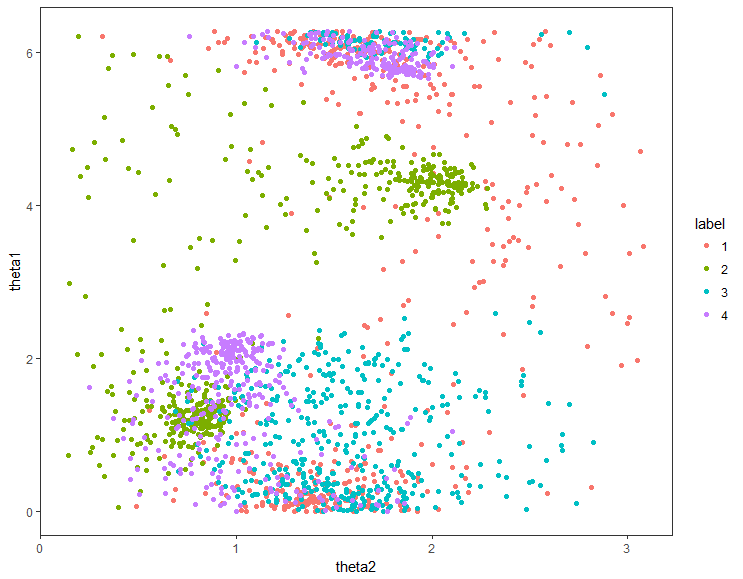
\includegraphics[clip,height= 45mm]{data/real.png}
\end{center}
\end{minipage}

\begin{minipage}{0.5\hsize}
\begin{center}
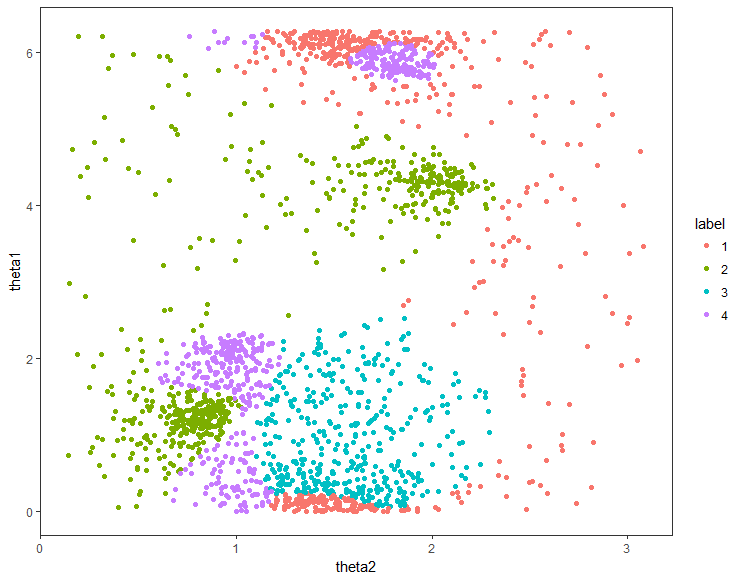
\includegraphics[clip,height= 45mm]{data/pred.png}
\end{center}
\end{minipage}
\end{tabular}
\caption{人工データの角度$\bm \theta = (\theta_1, \theta_2)^T$における散布図(左), 球面上の角度$\bm \theta = (\theta_1, \theta_2)^T$におけるクラスタリング結果(右)}
\end{figure}

\begin{itemize}
\item
複数のvon Mises 分布に従う乱数を発生させて, 1つのデータにまとめることで混合データを作成する.
\end{itemize}

\end{frame}

%%%%%%%%%  データ解析 %%%%%%%%%%%%
\section{データ解析}
\begin{frame}{解析データ}

本研究では, GroupLens による公開データセットMovieLensの一部分を用いた. MovieLensデータセットは映画評価サイト''movielens.com''において1997年9月から1998年4月までの7ヶ月間の間に集められた943人のユーザ, 1682個の映画についての10万個の評価値, 簡単なユーザ情報, コンテンツ情報から構成されている. 評価値において, $0$は見ていないことを表し, 評価については1から5までの5段階評価で数字が大きいほど高い評価である. 各ユーザは最低20個の映画に対する評価値を持っている. コンテンツ情報, ユーザ情報について表\ref{MovieLens1}にまとめる. また表\ref{MovieLens2}にMovieLensデータセットの一部を示す.


\begin{table}[bp]
\begin{center}
\caption{コンテンツ情報およびユーザ情報}   %キャプション
\label{MovieLens1}   %ラベル
\scalebox{0.7}{
\begin{tabular}{c l}
\hline
ジャンル & unknown, Action, Adventure, Animation, Children's, Comedy, \\
                 & Crime, Documentary, Drama, Fantasy, Film-Noir, Horror, Musical, \\
                 & Mystery, Romance, Sci-Fi, Thriller, War, Western \\
職業          & administrator, artist, doctor, educator, engineer, entertainment, executive, \\
                & healthcare, homemaker, lawyer, librarian, marketing, none, other, \\
                & programmer, retired, salesman, scientist, student, technician, writer \\
年齢 & 7歳 $\sim$ 73歳 \\
性別 & male, female\\ 
\hline
\end{tabular}
}
\end{center}
\end{table}

\end{frame}

\begin{frame}{データ解析(1/2)}

情報量基準(WAIC)を用いて, 混合分布のコンポーネントの選択を行う. AICやBICなどの情報量基準には, 事後分布が正規分布で近似されている必要があるなど, 様々な制約が存在するが, WAICは真の分布, 確率モデル, 事前分布がどのような場合でも用いることができる. WAICは式$(\ref{WAIC1})$で求められる.

\begin{eqnarray}
\label{WAIC1}
\mbox{WAIC} = T + \frac{V}{n}, 
\end{eqnarray}

\begin{table}[tbp]
\caption{WAICによるコンポーネントの選択結果}
\label{WAIC2}
\begin{center}
\scalebox{0.5}{
\begin{tabular}{l | c c c c c c c c c c}
\hline
 & 1 & 2 & 3 & 4 & 5 & 6 & 7 & 8 & 9 & 10 \\ \hline 
$m=1$ & -1014.1 & -1237.0 & -1350.6 & -1009.5 & -1308.8 & -1227.8 & -1152.4 & -902.5 & -1322.6 & -1140.2 \\ 
$m=2$ & -1610.9 & -1675.0 & -1760.4 & -1552.8 & -1633.1 & -1529.6 & -1507.1 & -1366.1 & -1645.2 & -1693.3 \\ 
$m=3$ & -1846.8 & -1744.7 & -1728.9 & -1804.9 & -1741.0 & -1654.3 & -1705.2 & -1633.8 & -1789.3 & \textbf{-1872.1} \\ 
$m=4$ & \textbf{-1893.6} & \textbf{-1969.8} & \textbf{-1901.6} & \textbf{-1837.5} & \textbf{-1787.5} & \textbf{-1687.8} &\textbf{-1749.5} & \textbf{-1686.7} & \textbf{-1844.5} & -1802.6 \\ 
\hline
\end{tabular}
}
\end{center}
\end{table}

\end{frame}

%%%%%%%%%%%%%% まとめと今後の課題 %%%%%%%%%%%%%%%%%
\section{まとめと今後の課題}
\begin{frame}{まとめと今後の課題}

\begin{itemize}

\item
前日と前々日の混合分布で今日の風向の分布を予測.

\item
少数のデータで分布の予測.

\end{itemize}

\end{frame}

\section{参考文献}
\begin{frame}[allowframebreaks]{参考文献}

{\scriptsize
\begin{thebibliography}{99}
%\setlength{\itemsep}{-.5zw}
\beamertemplatetextbibitems %参考文献に番号を振る

\bibitem{GPN}
D.Hernandez-Stumpfhauser and F. J. Breidt and Mark J. van der Woerd. (2017). The General Projected Normal Distribution of Arbitrary Dimension: Modeling and Bayesian Inference. {\it Journal of Bayesian Analysis}, Vol. 12, No. 1, pp. 113-133.

\bibitem{PN1}
F. Wang and A. E. Gelfand. (2013). Directional data analysis under the general
projected normal distribution. {\it Statistical Methodology}, Vol.10, pp. 113-127.

\bibitem{PN2}
B. Presnell, S. P. Morrison, and R. C. Littell. (1998). Projected multivariate linear models for
directional data. {\it Journal of the American Statistical Association}, Vol. 443, pp. 1068-1077.

%\bibitem{mvonMF}
%Jalil Taghia and Zhanyu Ma and Arne Leijon. (2014). Bayesian Estimation of the von-Mises Fisher Mixture %Model with Variational Inference. {\it IEEE}, Vol.36, No. 9, pp. 1701-1715.

\bibitem{vonMF}
S. Gopal and Y. Yang. (2014). Von Mises-Fisher Clustering Models. {\it ICML}.

\bibitem{skmeans}
S. Dhillon and S. Modha. (2001). Concept Decompositions for Large Sparse Text Data Using
Clustering. {\it Machine Learning}, Vol. 42, pp. 143-175.

\bibitem{movie}
GroupLensホームページ(http://movielens.org/.) 

\end{thebibliography}
}

\end{frame}
\end{document}

%\vspace{-0.5cm}
%\begin{figure}[H]
% \begin{center}
 % 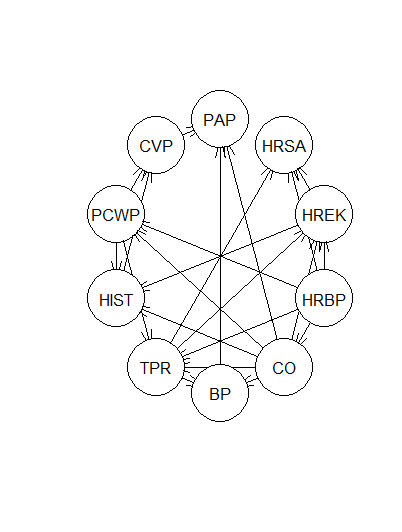
\includegraphics[width=40mm]{data/BN4.png}
 %\end{center}
 %\caption{ベイジアンネットワークの例}
 %\label{naive}
%\end{figure}